La tarea de análisis de un sistema conlleva la especificación de una serie 
de requisitos que guíen el posterior diseño e implementación del sistema 
\gls{MOLDEAS}, de esta forma, se pueden extraer los siguientes objetivos: 
\begin{itemize}
 \item Analizar e identificar el trabajo relacionado.
 \item Identificar y definir los requisitos asociados a las actividades de investigación, 
innovación y desarrollo a realizar.
 \item Realimentar los puntos anteriores con los resultados obtenidos.
\end{itemize}

Estos objetivos ya han sido parcialmente cubiertos en los anteriores 
capítulos, en los cuales se ha repasado intensivamente la mayor parte de los trabajos más relevantes relacionados con 
el dominio de la contratación pública electrónica, así como puesto de manifiesto los procesos, 
métodos y tareas a desarrollar dentro del ciclo de vida de datos 
enlazados. Es por ello que este capítulo se centrará en presentar las partes más prominentes y 
destacadas del sistema MOLDEAS y su aplicación en las distintas 
tareas del ciclo de vida, así como en el desarrollo del sistema de búsqueda 
de anuncios de licitación. En primer lugar, cabe mostrar un esbozo del 
sistema con una vista funcional del mismo, ver Figura~\ref{fig:functional-overview}, en el cual 
se enclavan los distintos procesos del ciclo de vida y los objetivos generales del sistema: 
producción de datos enlazados de los anuncios de licitación para su posterior 
almacenamiento y publicación a través de un \textit{endpoint} de \gls{SPARQL} y un \linkeddata \textit{frontend} y 
consumo de los datos almacenados para la construcción de servicios de valor añadido como el 
sistema de búsqueda/recomendación de anuncios de licitación. Se ha optado por un enfoque 
totalmente práctico en este capítulo de ingeniería con el objetivo de resaltar y documentar la innovación del sistema 
MOLDEAS sin focalizar en metodologías intensivas de ingeniería del \textit{software}.


\begin{figure}[!htb]
\centering
	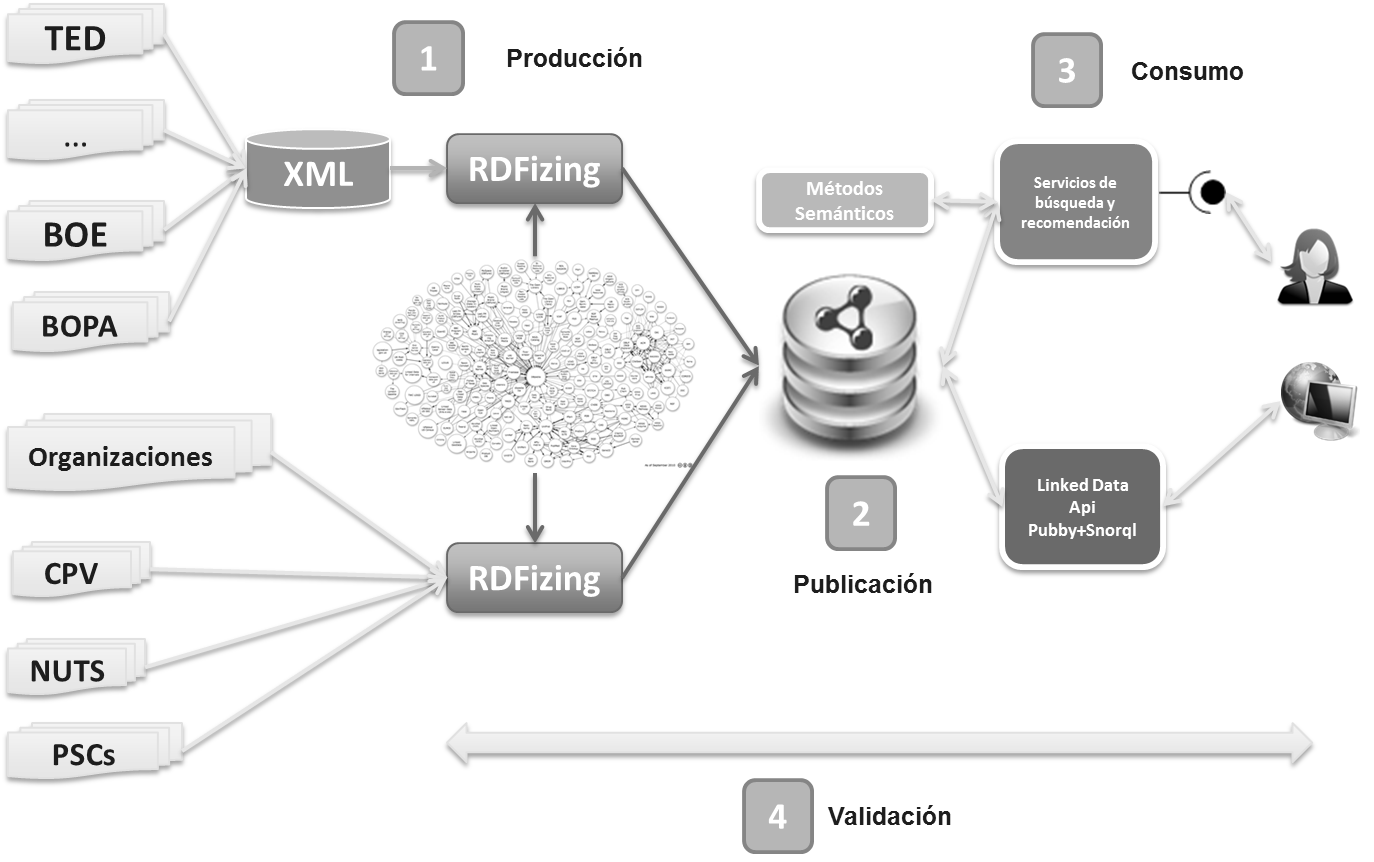
\includegraphics[width=12cm]{images/phd/moldeas/functional-overview}
\caption{Arquitectura funcional del sistema MOLDEAS.}
\label{fig:functional-overview}
\end{figure}

A la vista de la arquitectura funcional propuesta, se ha realizado una aproximación en distintos componentes, 
de acuerdo a sus responsabilidades e interacciones, ver Figura~\ref{fig:moldeas-components}, y con las siguientes 
definiciones:

\begin{description}
 \item [moldeas-common.] Alberga utilidades necesarias a lo largo de todos los procesos del ciclo de vida de datos 
enlazados.
 \item [moldeas-transformer.] Se encarga de dar soporte a la producción de datos enlazados cubriendo las tareas de transformación, 
  enriquecimiento, reconciliación de entidades, etc.  
 \item [moldeas-api.] Se encarga del consumo de los datos enlazados publicados bajo unas 
ciertas características en un \textit{endpoint} de SPARQL y que con la aplicación de varios 
métodos de expansión de consultas es capaz de generar consultas SPARQL cercanas al lenguaje natural 
para la recuperación de los anuncios de licitación.
\item [moldeas-test.] Se encarga de la validación de los datos enlazados y de los métodos de expansión definidos en \texttt{moldeas-api}.
 \item [moldeas-web.] Se encarga de la presentación y consumo de datos enlazados suministrando 
un interfaz gráfico para \texttt{moldeas-api} en el cual el usuario puede seleccionar las 
características de los anuncios de licitación para su posterior búsqueda y 
presentación con diferentes vistas (tabla, mapa, etc.). Además, suministra un interfaz de servicios REST para el acceso 
a los métodos disponibles en \texttt{moldeas-api}, por lo que cumple una doble función: 1) servir como demostrador 
público para el usuario y 2) ejemplificar las llamadas a \texttt{moldeas-api} desde un punto de vista 
del desarrollador.
\end{description}

\begin{figure}[!htb]
\centering
	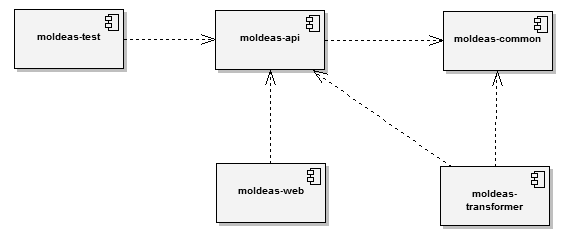
\includegraphics[width=12cm]{images/phd/moldeas/moldeas-componentes}
\caption{Componentes del sistema MOLDEAS.}
\label{fig:moldeas-components}
\end{figure}

\subsection{Arquitectura de alto nivel}
%Diagramas de componentes, diagramas de paquetes
El despliegue de una infraestructura de datos enlazados requiere la cooperación de diferentes elementos 
\textit{hardware} y \textit{software}. Según el análisis realizado de cada uno de los componentes un diagrama 
de despliegue de la arquitectura propuesta en MOLDEAS, se presenta en la Figura~\ref{fig:moldeas-despliegue}, la descripción de cada uno de estos nodos y componentes es la siguiente:

\begin{itemize}

\item Nodo web. En el cual se encuentran disponibles un servidor web \gls{HTTP}, Apache2 HTTP Server, este elemento \textit{software} sirve como punto 
de entrada a los elementos del sistema, tanto para el consumo de datos enlazados directamente por otras máquinas como para las peticiones 
relativas al componente \texttt{moldeas-web}. También, se utiliza este servicio para albergar una aplicación 
de ejecución de consultas \textit{on-line} en SPARQL como \gls{SNORQL}, sin necesidad de utilizar directamente 
el interfaz propuesto por el \textit{endpoint} de SPARQL.

\item Nodo de aplicaciones web. En el cual se encuentra instalado un contenedor de aplicaciones web \gls{J2EE} como Apache Tomcat, 
con el objetivo de albergar las aplicaciones relativas al \linkeddata \textit{frontend} y a la aplicación \texttt{moldeas-web}. 

\item Nodo repositorio RDF. En el cual se instala el repositorio \gls{RDF}, en el cual se almacenan y publican 
los datos enlazados provenientes de los anuncios de licitación. La publicación de datos enlazados se realiza a través de su almacenamiento 
en un repositorio RDF nativo como Virtuoso de OpenLink, suministrando adicionalmente un \textit{endpoint} SPARQL para que los 
datos puedan ser reutilizados y consumidos tanto por la propia aplicación de \texttt{moldeas-api} como por clientes 
de forma externa, en este caso por el \linkeddata \textit{frontend} y SNORQL.

\end{itemize}

Físicamente estos nodos y componentes se han diseñado de forma separada ya que la comunicación entre los mismos 
se realiza mediante delegación de consultas y comunicación mediante HTTP. De esta manera, se permite que el sistema 
sea escalable y flexible, pudiendo sustituir el entorno tecnológico seleccionado por otros proveedores.

Los componentes especificados en MOLDEAS tienen un doble carácter ya que algunos son utilizados de forma \textit{off-line} como 
es el caso de \texttt{moldeas-transformer} y \texttt{moldeas-test}, específicamente para los procesos de producción y validación 
de datos enlazados, mientras que otros como \texttt{moldeas-web} sirven como cliente de los servicios proporcionados 
en \texttt{moldeas-api} de forma \texttt{on-line}. Transversalmente \texttt{moldeas-common} se utiliza a lo largo de cualquier 
ejecución ya que contiene las clases \textit{Helper} necesarias para la ejecución de tareas comunes.

\begin{figure}[!htb]
\centering
	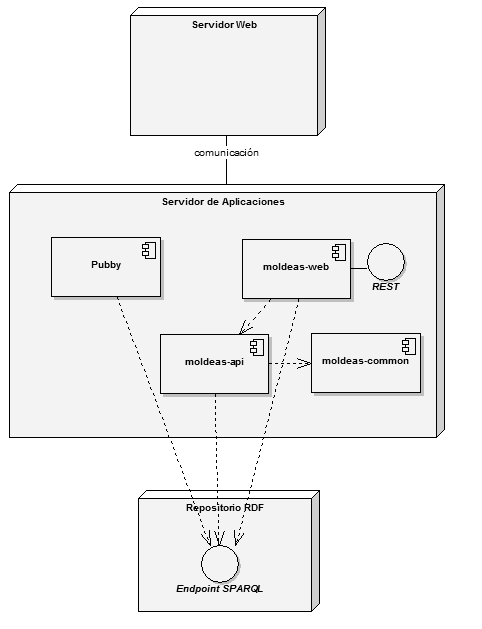
\includegraphics[width=12cm]{images/phd/moldeas/moldeas-despliegue}
\caption{Diagrama de Despliegue de MOLDEAS.}
\label{fig:moldeas-despliegue}
\end{figure}

\subsection{Entorno Tecnológico}
En el momento de analizar y diseñar un conjunto de componentes \textit{software} es necesario seleccionar aquellas 
bibliotecas y herramientas que suministren determinadas funcionalidades de base. La selección estratégica 
de esta tecnología y herramientas se describe someramente a continuación:

\begin{itemize}
 \item Lenguaje de programación Java 1.6. En el campo de la Web Semántica y en particular de la iniciativa de 
datos enlazados, la mayoría de las bibliotecas y funcionalidades externas se encuentran programadas 
en este lenguaje, este hecho unido a la experiencia propia del autor, justifica perfectamente la decisión de uso de este lenguaje.
\item Apache Maven2. El desarrollo de aplicaciones debe realizarse de forma sostenible, es por ello que esta herramienta da 
soporte a todo el proceso de construcción de \textit{software}: compilación, pruebas, empaquetado, despliegue, documentación, ejecución, etc. 
Además de proveer los mecanismos apropiados para la gestión de dependencias de forma declarativa. 
\item Eclipse \gls{IDE}. La edición del código fuente de las clases Java se ha realizado a través de este entorno de desarrollo, ampliamente 
asentado en la comunidad Java y con una excelente comunidad que proporciona herramientas extra a través de distintos 
\textit{plugins}, proporcionando un entorno productivo y con altas capacidades para el desarrollador. Adicionalmente, Maven 
es capaz de generar a través de su fichero de configuración la estructura de un  proyecto de Eclipse de forma automática.
\item Repositorio de código fuente. Se ha seleccionado la forja de proyectos de Google Code para albergar los cambios y las actualizaciones 
maduras a través del sistema de control de versiones Mercurial.
\item Jena 2.6.4. Biblioteca Java de base tecnológica para la Web Semántica que incluye las principales funciones para el tratamiento de \gls{RDF}, \gls{OWL}, 
etc., facilitando la ejecución de consultas \gls{SPARQL} tanto de forma local (en memoria) como distribuida (en un \textit{endpoint}).
\item Log4j 1.2.14. Biblioteca Java para la gestión del sistema de registro de una aplicación mediante la cual se puede especificar 
los distintos niveles de registro así como la serialización de los mismos.
\item Junit 4.0. \textit{Framework} Java para la ejecución de pruebas unitarias con un amplio abanico de configuraciones y extras 
para el diseño de pruebas de integración, regresión, etc.
\item Apache \gls{Lucene} 2.9.0. Motor de búsqueda sintáctica en Java con amplias posibilidades tanto para el indexado de documentos, procesamiento 
de lenguaje natural y ejecución de consultas.
\item Apache \gls{Solr} 1.4.1. Plataforma empresarial de búsqueda en Java basada en Apache Lucene que añade nuevas funcionales como nuevos 
filtros para el procesamiento de lenguaje natural.
\item Apache \gls{Mahout} 0.4. Biblioteca Java con un amplio espectro de algoritmos de \textit{data mining} y aprendizaje automático, con capacidades 
para integrarse con otras herramientas como Apache Hadoop y que propone un framework extensible para la creación de nuevos algoritmos.
\item Spring 2.5. \textit{Framework} Java para la creación de aplicaciones empresariales basado en la técnica inversión de control y el uso 
de \textit{Plain Old Java Object} (\gls{POJO}s) para el diseño flexible y el desarrollo ágil de \textit{software}.
\item Jersey \gls{REST} 0.8. Biblioteca Java para la creación de servicios web REST mediante anotaciones.
\item Jquery 1.4.1. \textit{Framework} para el desarrollo de interfaces de usuario enriquecidos basados en HTML+CSS+Javascript.
\item Exhibit 2.2.0. Biblioteca basada en Javascript para el desarrollo de interfaces con múltiples vistas para la presentación 
de datos en general.
\item \gls{Pubby} 0.3.3. \linkeddata \textit{frontend} para la negociación de contenido y presentación de datos enlazados disponibles 
a través de un \textit{endpoint} de \gls{SPARQL}.
\item \gls{SNORQL}. Aplicación basada en HTML+Javascript para la realización de consultas \textit{on-line} sobre \textit{endpoints} de SPARQL.

\end{itemize}



















